\section{Linear Transformations}

\begin{frame}{Linear Transformations}
    \begin{itemize}
        \item \textbf{Linear transformations} are operations that can be performed by applying a matrix to a vector. 
        \item Some common transformations include \textbf{rotation} and \textbf{reflection}.
    \end{itemize}
    \begin{center}
        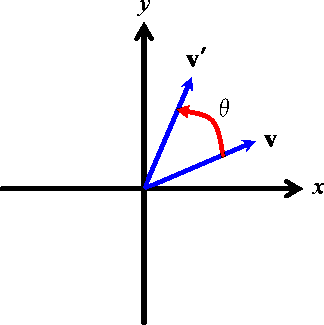
\includegraphics[width = 0.45\textwidth]{images/vector-rotation.png} 
        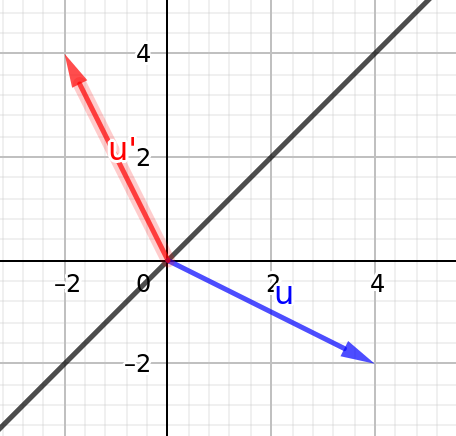
\includegraphics[width = 0.45\textwidth]{images/vector-reflection.png}
    \end{center}
\end{frame}

\begin{frame}{Common Linear Transformations: Rotation}
    The \textbf{rotation matrix} rotates points by a specific angle, $\theta$:
    \begin{align*}
        R(\theta) = \begin{bmatrix} 
                \cos(\theta) & -\sin(\theta) \\
                \sin(\theta) & \cos(\theta)
            \end{bmatrix}
    \end{align*}
    Use this matrix by \textbf{plugging in the desired rotation angle}, then multiply it to a vector.
    \begin{align*}
        R(\theta) = \begin{bmatrix} 
            0 & -1 \\
            1 & 0
        \end{bmatrix}
    \end{align*}
    Rotation matrices also \textbf{preserve the length} of a vector. Check it! (\textit{Think about the eigenvalues! Real? Complex? How about the magnitude of these eigenvalues?})
\end{frame}

\begin{frame}{Common Linear Transformations: Reflection}
    \begin{itemize}
        \item The reflection matrix \textbf{reflects vectors} across a line. (Notice that such matrix also \textit{preserves the length of a vector}.)
        \item Notable reflection matrices:
        \begin{itemize}
            \item Reflection across x-axis: $\begin{bmatrix} 1 & 0 \\ 0 & -1 \end{bmatrix}$ \\[1.1ex]
            \item Reflection across y-axis: $\begin{bmatrix} -1 & 0 \\ 0 & 1 \end{bmatrix}$ \\[1.1ex]
            \item Reflection across line $y = x$: $\begin{bmatrix} 0 & 1 \\ 1 & 0 \end{bmatrix}$
        \end{itemize}
    \end{itemize}
\end{frame}

\begin{frame}{Practice: Matrix Transformations}
    Create matrices to transform the vector $\vec{v} = \begin{bmatrix} 2 & 3 \end{bmatrix}^T$ as follows:
    \begin{enumerate}
        \item Rotate by $45\deg$
        \item Reflect across $y = x$
    \end{enumerate}
\end{frame}

\begin{frame}{Practice: Matrix Transformations}
    Create matrices to transform the vector $\vec{v} = \begin{bmatrix} 2 & 3 \end{bmatrix}^T$ as follows:
    \begin{enumerate}
        \item Rotate by $45\deg$
        \begin{align*}
            \begin{bmatrix}
                \frac{\sqrt{2}}{2} & -\frac{\sqrt{2}}{2} \\[0.8ex]
                \frac{\sqrt{2}}{2} & \frac{\sqrt{2}}{2}
            \end{bmatrix}
            \begin{bmatrix} 
                2 \\ 3 
            \end{bmatrix} = 
            \begin{bmatrix} 
                -\frac{\sqrt{2}}{2} \\[0.8ex] \frac{5\sqrt{2}}{2}
            \end{bmatrix}
        \end{align*}
        \item Reflect across $y = x$
        \begin{align*}
            \begin{bmatrix}
                0 & 1 \\
                1 & 0
            \end{bmatrix}
            \begin{bmatrix}
                2 \\ 3
            \end{bmatrix} = 
            \begin{bmatrix}
                3 \\ 2
            \end{bmatrix}
        \end{align*}
    \end{enumerate}
\end{frame}